\documentclass[tikz,border=10pt]{standalone}
\usepackage{tikz,amsmath}
\usetikzlibrary{arrows.meta,positioning,calc,fit}
\begin{document}
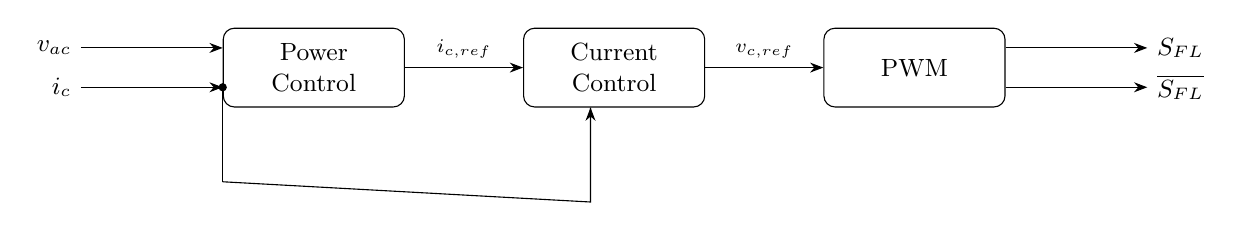
\begin{tikzpicture}[
  font=\small,
  >=Stealth,
  block/.style={draw, rounded corners, minimum width=2.3cm, minimum height=1.0cm, align=center},
  dot/.style={circle, fill=black, inner sep=0pt, minimum size=3pt},
]

% Blocks
\node[block]                        (PC)   at (0, 0)   {Power\\Control};
\node[block, right=1.5cm of PC]     (CC)              {Current\\Control};
\node[block, right=1.5cm of CC]     (PWM)             {PWM};

% Input signals on the left, entering horizontally
\coordinate (vac_in) at ($(PC.west) + (-1.8, 0.25)$);
\coordinate (ic_in)  at ($(PC.west) + (-1.8, -0.25)$);
\node[left] at (vac_in) {$v_{ac}$};
\node[left] at (ic_in)  {$i_c$};
\draw[->] (vac_in) -- ($(PC.west) + (0, 0.25)$);
\draw[->] (ic_in)  -- ($(PC.west) + (0, -0.25)$) coordinate (PCin_i);

% i_c splits to feed Current Control too (dot at branch)
\node[dot] at (PCin_i) {};
\draw (PCin_i) -- ++(0, -1.2) coordinate (ibus);
\draw (ibus) -- ($(CC.south) + (-0.3, 0) - (0, 1.2)$) -- ($(CC.south) + (-0.3, 0)$);
\draw[->] ($(CC.south) + (-0.3, 0) - (0, 1.2)$) -- ($(CC.south) + (-0.3, 0)$);

% PC -> CC
\draw[->] (PC) -- node[above, font=\scriptsize]{$i_{c,ref}$} (CC);

% CC -> PWM
\draw[->] (CC) -- node[above, font=\scriptsize]{$v_{c,ref}$} (PWM);

% PWM outputs
\coordinate (sfl_out) at ($(PWM.east) + (1.8, 0.25)$);
\coordinate (ssl_out) at ($(PWM.east) + (1.8, -0.25)$);
\draw[->] ($(PWM.east) + (0, 0.25)$)  -- (sfl_out);
\draw[->] ($(PWM.east) + (0, -0.25)$) -- (ssl_out);
\node[right] at (sfl_out) {$S_{FL}$};
\node[right] at (ssl_out) {$\overline{S_{FL}}$};

\end{tikzpicture}
\end{document}
